\documentclass[tikz,border=2pt]{standalone}
\usepackage{amsmath,amssymb}
\usepackage{tikz}
\usetikzlibrary{arrows.meta}

\begin{document}
% A Jordan chain: repeatedly applying (A - lambda I) walks a generalized eigenvector down to
% an ordinary eigenvector and then to 0.
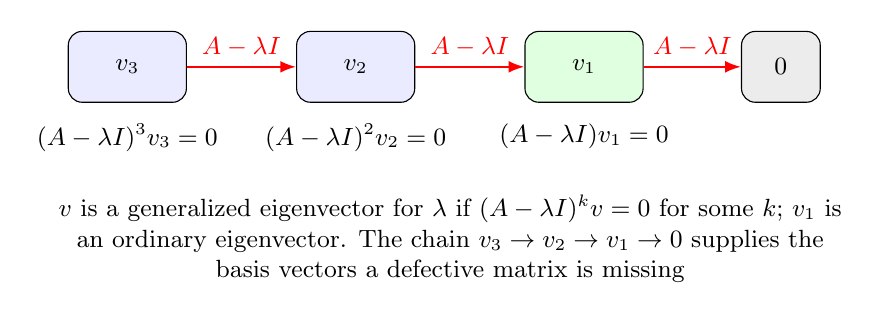
\begin{tikzpicture}[every node/.style={font=\small}, >={Latex[length=2mm]}]
	\node[draw, rounded corners=5pt, fill=blue!8, minimum width=1.5cm, minimum height=0.9cm] (v3) at (0,0) {$v_3$};
	\node[draw, rounded corners=5pt, fill=blue!8, minimum width=1.5cm, minimum height=0.9cm] (v2) at (2.9,0) {$v_2$};
	\node[draw, rounded corners=5pt, fill=green!12, minimum width=1.5cm, minimum height=0.9cm] (v1) at (5.8,0) {$v_1$};
	\node[draw, rounded corners=5pt, fill=gray!15, minimum width=1.0cm, minimum height=0.9cm] (z) at (8.3,0) {$0$};
	\draw[->, thick, red] (v3) -- (v2) node[midway, above] {$A-\lambda I$};
	\draw[->, thick, red] (v2) -- (v1) node[midway, above] {$A-\lambda I$};
	\draw[->, thick, red] (v1) -- (z) node[midway, above] {$A-\lambda I$};
	\node[font=\small, anchor=north] at (0,-0.6) {$(A-\lambda I)^3v_3=0$};
	\node[font=\small, anchor=north] at (2.9,-0.6) {$(A-\lambda I)^2v_2=0$};
	\node[font=\small, anchor=north] at (5.8,-0.6) {$(A-\lambda I)v_1=0$};
	\node[anchor=north, align=flush center, text width=10cm] at (4.1,-1.5) {$v$ is a generalized eigenvector for $\lambda$ if $(A-\lambda I)^kv=0$ for some $k$; $v_1$ is an ordinary eigenvector. The chain $v_3\to v_2\to v_1\to0$ supplies the basis vectors a defective matrix is missing};
\end{tikzpicture}
\end{document}
